\documentclass[]{article}


%\usepackage{pdfpages}
\usepackage{url}

\usepackage{amsmath}
\usepackage{amsfonts}
\usepackage{amssymb}
\usepackage{caption}
\usepackage{cite}
\usepackage{comment}
\usepackage{color}
\usepackage{enumerate}
\usepackage{graphicx}
\usepackage[hidelinks]{hyperref}
\usepackage{listings}
\usepackage{natbib}
\usepackage{pgfplots}
\usepackage{subcaption}
\usepackage{tikz}
\usepackage{titlesec}
\usepackage{verbatim}
\usepackage{xcolor}

\title{Variational Autoencoders - Notes}
\author{Anna-Lena Popkes}

\begin{document}

\maketitle

\section{Variational Inference}
\label{sec:variational_inference}

\begin{itemize}
    \item Variational Bayesian methods are a family of techniques for approximating intractable integrals arising in Bayesian inference and machine learning
    \item They are typically used in complex statistical models consisting of observed variables (data) as well as unknown parameters and latent variables
        \item Variational Bayesian methods are primarily used for two purposes:
        \begin{enumerate}
        	\item To provide an approximation to the posterior probability of the unobserved variables, in order to do statistical inference over these variables
        	\item To derive a lower bound for the marginal likelihood (evidence) of the observed data (i.e. the marginal probability of the data given the model, with marginalization performed over unobserved variables). 
        	
        \end{enumerate}
	\item We want to estimate the posterior distribution $p(z|x)$. However, for many models the exact posterior cannot be computed
    \item In variational inference, the posterior distribution over a set of unobserved variables $z_1, ..., z_n$ given some data $x$ is approximated by a \textit{variational} \textit{distribution} $q(z)$: $p(z|x) \approx q(z)$ 
    \item The distribution $q(z)$ is restricted to belong to a family of distributions of simpler form than $p(z|x)$
    \item $q(z)$ should be as similar to the true posterior $p(z|x)$ as possible
    \item This is done by finding a setting of the parameters that makes $q$ as close to the true posterior as possible
    \item The dissimilarity between the two distributions is typically measured using the Kullback-Leipler divergence $D_{KL}(q(z)||p(z|x))$
    \item The KL divergence can't be minimized exactly. But we can minimize a function that is equal to it up to a constant. This is the \textit{evidence} \textit{lower} \textit{bound}  (ELBO)
   \item We reformulate the KL divergence as follows:\\
    $D_{KL}(q(z)||p(z|x)) = \mathbb{E}_q \Big[ \log \frac{q(z)}{p(z|x)} \Big] \\ = -\mathbb{E}_q \big[ \log p(z,x) \big] + \mathbb{E}_q \big[\log q(z) \big] + \log p(x) $
   \item  This is the negative ELBO plus the log marginal probability of x
   \item Maximizing the ELBO is equivalent to minimizing the KL divergence

\end{itemize}


\section{Optimization algorithms}

This section introduces the major optimization algorithms that use adaptive learning rates for the parameters in a model. All figures come from source 2.

\subsection{AdaGrad}
\begin{itemize}
	\item Individually adapts the learning rates of all model parameters by scaling them inversely proportional to the square root of the sum of all their historical squared values (see figure \ref{fig:adagrad})
	\item Therefore, parameters with large partial derivatives have a higher decrease in their learning rate
	\item Parameters with small partial derivatives have a smaller decrease in their learning rate
\end{itemize}

\begin{figure}[h!]
	\centering
	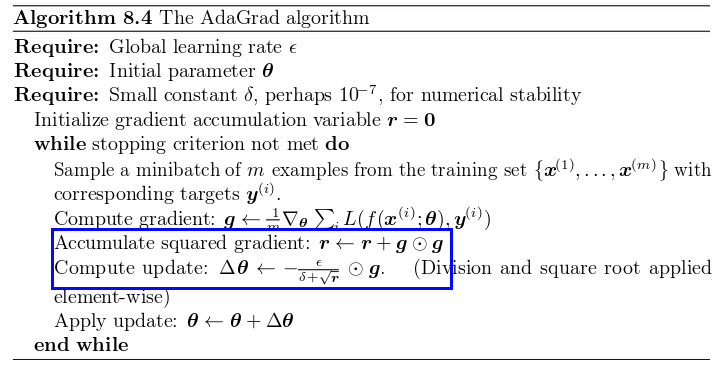
\includegraphics[width=0.8\linewidth]{ada_grad}
	\caption{The AdaGrad algorithm}
	\label{fig:adagrad}
\end{figure}

\noindent For the training of deep networks it has been shown that accumulating squared gradients from the beginning of training can decrease learning rates too much and too quickly. 


\subsection{RMSProp}

Modifies AdaGrad and changes the gradient accumulation into an exponentially weighted moving average. This enables RMSProp to discard history from the extreme past. It can be used with or without Nesterov momentum. Figure \ref{fig:rms_prop} displays the algorithm without Nesterov momentum.

\begin{figure}[h!]
	\centering
	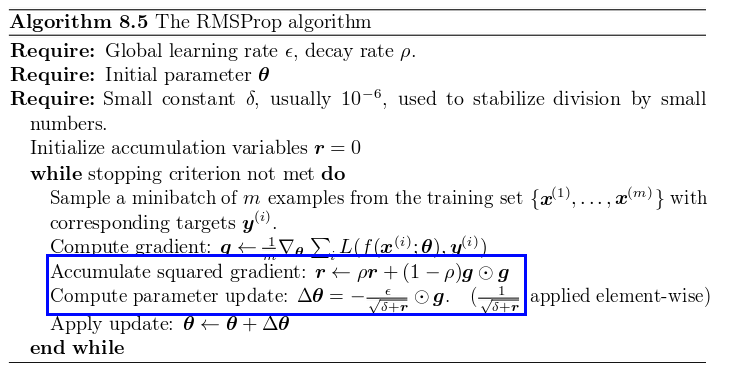
\includegraphics[width=0.8\linewidth]{rms_prop}
	\caption{The RMS algorithm}
	\label{fig:rms_prop}
\end{figure}

\noindent RMSProp has been shown to be both effective and practical for training deep networks.

\subsection{Adam}






\subsection{Sources}

\begin{enumerate}
	\item \url{http://sebastianruder.com/optimizing-gradient-descent/index.html#adagrad}
	\item \url{http://www.deeplearningbook.org/contents/optimization.html#pf23}
	
\end{enumerate}







\section{Variational Autoencoders}

\subsection{Basic Problem Setup}
\label{sec:vae_objective}

\begin{itemize}
    \item We are given a dataset of observations $x_1, ..., x_n$
    \item And a set of latent variables $z_1, ...., z_m$ with $z_i \sim p(z)$ 
    \item In variational autoencoders (VAEs) $p(z)$ is specified as a standard Normal distribution with mean zero and variance one, so $p(z) = \mathcal{N}(0,1)$
        \item The goal is to 
        
        
\end{itemize}

\subsection{Structure}
\label{}

\begin{itemize}
    \item A VAE consists of two parts
        \begin{enumerate}
        \item A probabilistic encoder $q_{\phi}(z|x)$ approximating the true but intractable posterior distribution $p(z|x)$
    \item A generative decoder $p_{\theta}(x|z)$ which does not rely on any particular input x
        \end{enumerate}
    \item The encoder is known as the \textit{inference} or \textit{recognition network}
        \item The decoder is known as the \textit{generative network}  
    \item Both the encoder and decoder are implemented as neural networks with tunable parameters $\theta$ and $\phi$
    \item For example, for $q_{\phi}(z|x)$ the neural network with parameters $\theta$ receives the input $x$ and produces $\mu, \Sigma$ as an output, e.g. $q_{\theta}(z|x) = \mathcal{N}(z| \mu(x, \theta),\Sigma(x, \theta))$. From this distribution we can draw samples of $z$, i.e. $z \sim q_{\phi}(z|x)$. 
    \item $p_{\theta}(x|z)$ is implemented in the same fashion
                \item Different to the classical autoencoder, we do not have a deterministic $z$ but we draw a random sample of $z$ from $q_{\phi}(z|x)$, i.e. $z$ is stochastic 
\end{itemize}

\begin{figure}[h!]
    \centering
    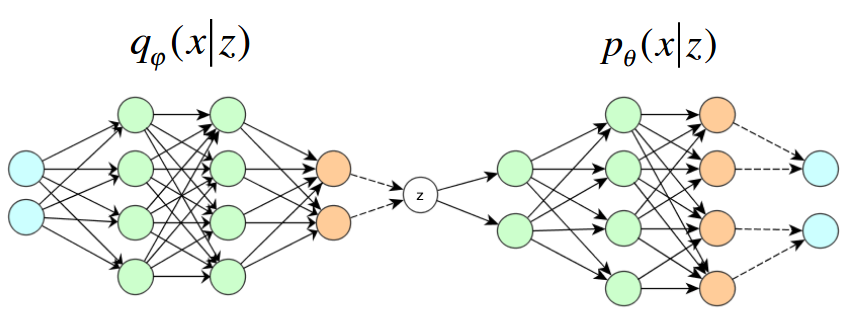
\includegraphics[width=0.8\linewidth]{VAE_parts}
    \caption{Encoding and decoding part of a VAE}
    \label{fig:vae}
\end{figure}

%\newpage

\subsection{Training}
\label{sec:vae_training}

\begin{itemize}
    \item Training a VAE or, more generally, a generative model, is the same as learning the joint distribution $p(x,z)$ over the data and latent variables
    \item We can write the joint probability distribution as $p(x,z) = p(x|z) p(z)$  
    \item In inference, the goal is to infer good values of the latent variables given the observed data. So we want to calculate $p(z|x) = \frac{p(x,z)}{p(x)} = \frac{p(x|z)p(z)}{p(x)}$ 
    \item $p(x)$ is called the evidence and can be calculated by marginalizing out the latent variables: $\int p(x|z) p(z) dz$
    \item We cannot compute this integral. Therefore, we approximate $p(z|x)$ with a family of distributions $q_{\phi}(z|x)$
    \item The variational parameter $\phi$ indexes the family of distributions. If $q$ were Gaussian, $\phi$ would be the mean and variace of the latent variables for each datapoint
    \item Our goal is to find the variational parameters $\phi$ that minimize the KL divergence between $q_{\phi}(z|x)$ and $p(z|x)$
    \item So we want to compute $\text{arg min}_q \text{ KL}(q_{\phi}(z|x)|| p(z|x))$
    \item As mentioned before, we cannot minimize KL directly. Therefore, we instead maximize the ELBO 
    \item The ELBO for a single datapoint $x_i$ is given by: \\ $ELBO(\phi, \theta) = \mathbb{E}_{q_{\phi}(z|x_i)} \big[\log p(x_i|z)\big] - D_{KL}(q_{\phi}(z|x_i)||p(z))$
    \item The ELBO rewards a good reconstruction (first term). The second term represents a regularizer that prevents col1=111xubuntuxubuntu
    xubuse ubuntu onuse ubutnlapsing to the deterministic autoencoder 
        
    \item The parameters $\phi, \theta$ are learned by maximizing this quantity using gradient descent and backpropagation
\end{itemize}

\subsection{Reparametrization Trick}
\label{sec:reparametrization_trick}

\subsection{Applications}
\begin{itemize}
	\item Analysis of brain MRI images:\\
	\url{http://www.cs.unc.edu/~eunbyung/papers/manifold_variational.pdf}
	
	\item Adversarial autoencoders:\\
	\url{https://arxiv.org/pdf/1511.05644.pdf}
	
	\item Sentence generation using an RNN-based VAE:\\
	\url{https://arxiv.org/pdf/1511.06349.pdf?TB_iframe=true&width=921.6&height=921.6}
	
	\item Predict the trajectory of pixels in scenes:\\
	\url{https://arxiv.org/pdf/1606.07873.pdf}
	
	\item Anomaly detection using a VAE+ESN:\\
	\url{http://ieeexplore.ieee.org/document/7727309/?reload=true}
	
	\item Anomaly detection:\\
	\url{http://dm.snu.ac.kr/static/docs/TR/SNUDM-TR-2015-03.pdf} 
	
	\item Adversarial autoencoder:\\
	\url{https://blog.paperspace.com/adversarial-autoencoders-with-pytorch/}
\end{itemize}


\subsection{Sources}
\label{sec:sources}
\begin{itemize}
    \item \url{https://www.cs.princeton.edu/courses/archive/fall11/cos597C/lectures/variational-inference-i.pdf})
    \item \url{https://home.zhaw.ch/~dueo/bbs/files/vae.pdf}
    \item \url{https://arxiv.org/pdf/1601.00670.pdf}
    \item \url{https://www.youtube.com/watch?v=lG1AIqIEv9I&index=3&list=PLR6O_WZHBlOE6xgFU725tenJszVDDHZyH}
    \item \url{https://jaan.io/what-is-variational-autoencoder-vae-tutorial/}
    \item \url{http://stats.stackexchange.com/questions/199605/how-does-the-reparameterization-trick-for-vaes-work-and-why-is-it-important}
    \item \url{http://dpkingma.com/wordpress/wp-content/uploads/2015/12/talk_nips_workshop_2015.pdf}
    \item \url{https://github.com/oduerr/dl_tutorial/blob/master/tensorflow/vae/vae_demo.ipynb}
    \item \url{https://jmetzen.github.io/2015-11-27/vae.html}
    \item \url{http://int8.io/variational-autoencoder-in-tensorflow/}  
     
        
        
        
\end{itemize}

\end{document}


